\begin{figure}
    \begin{center}
    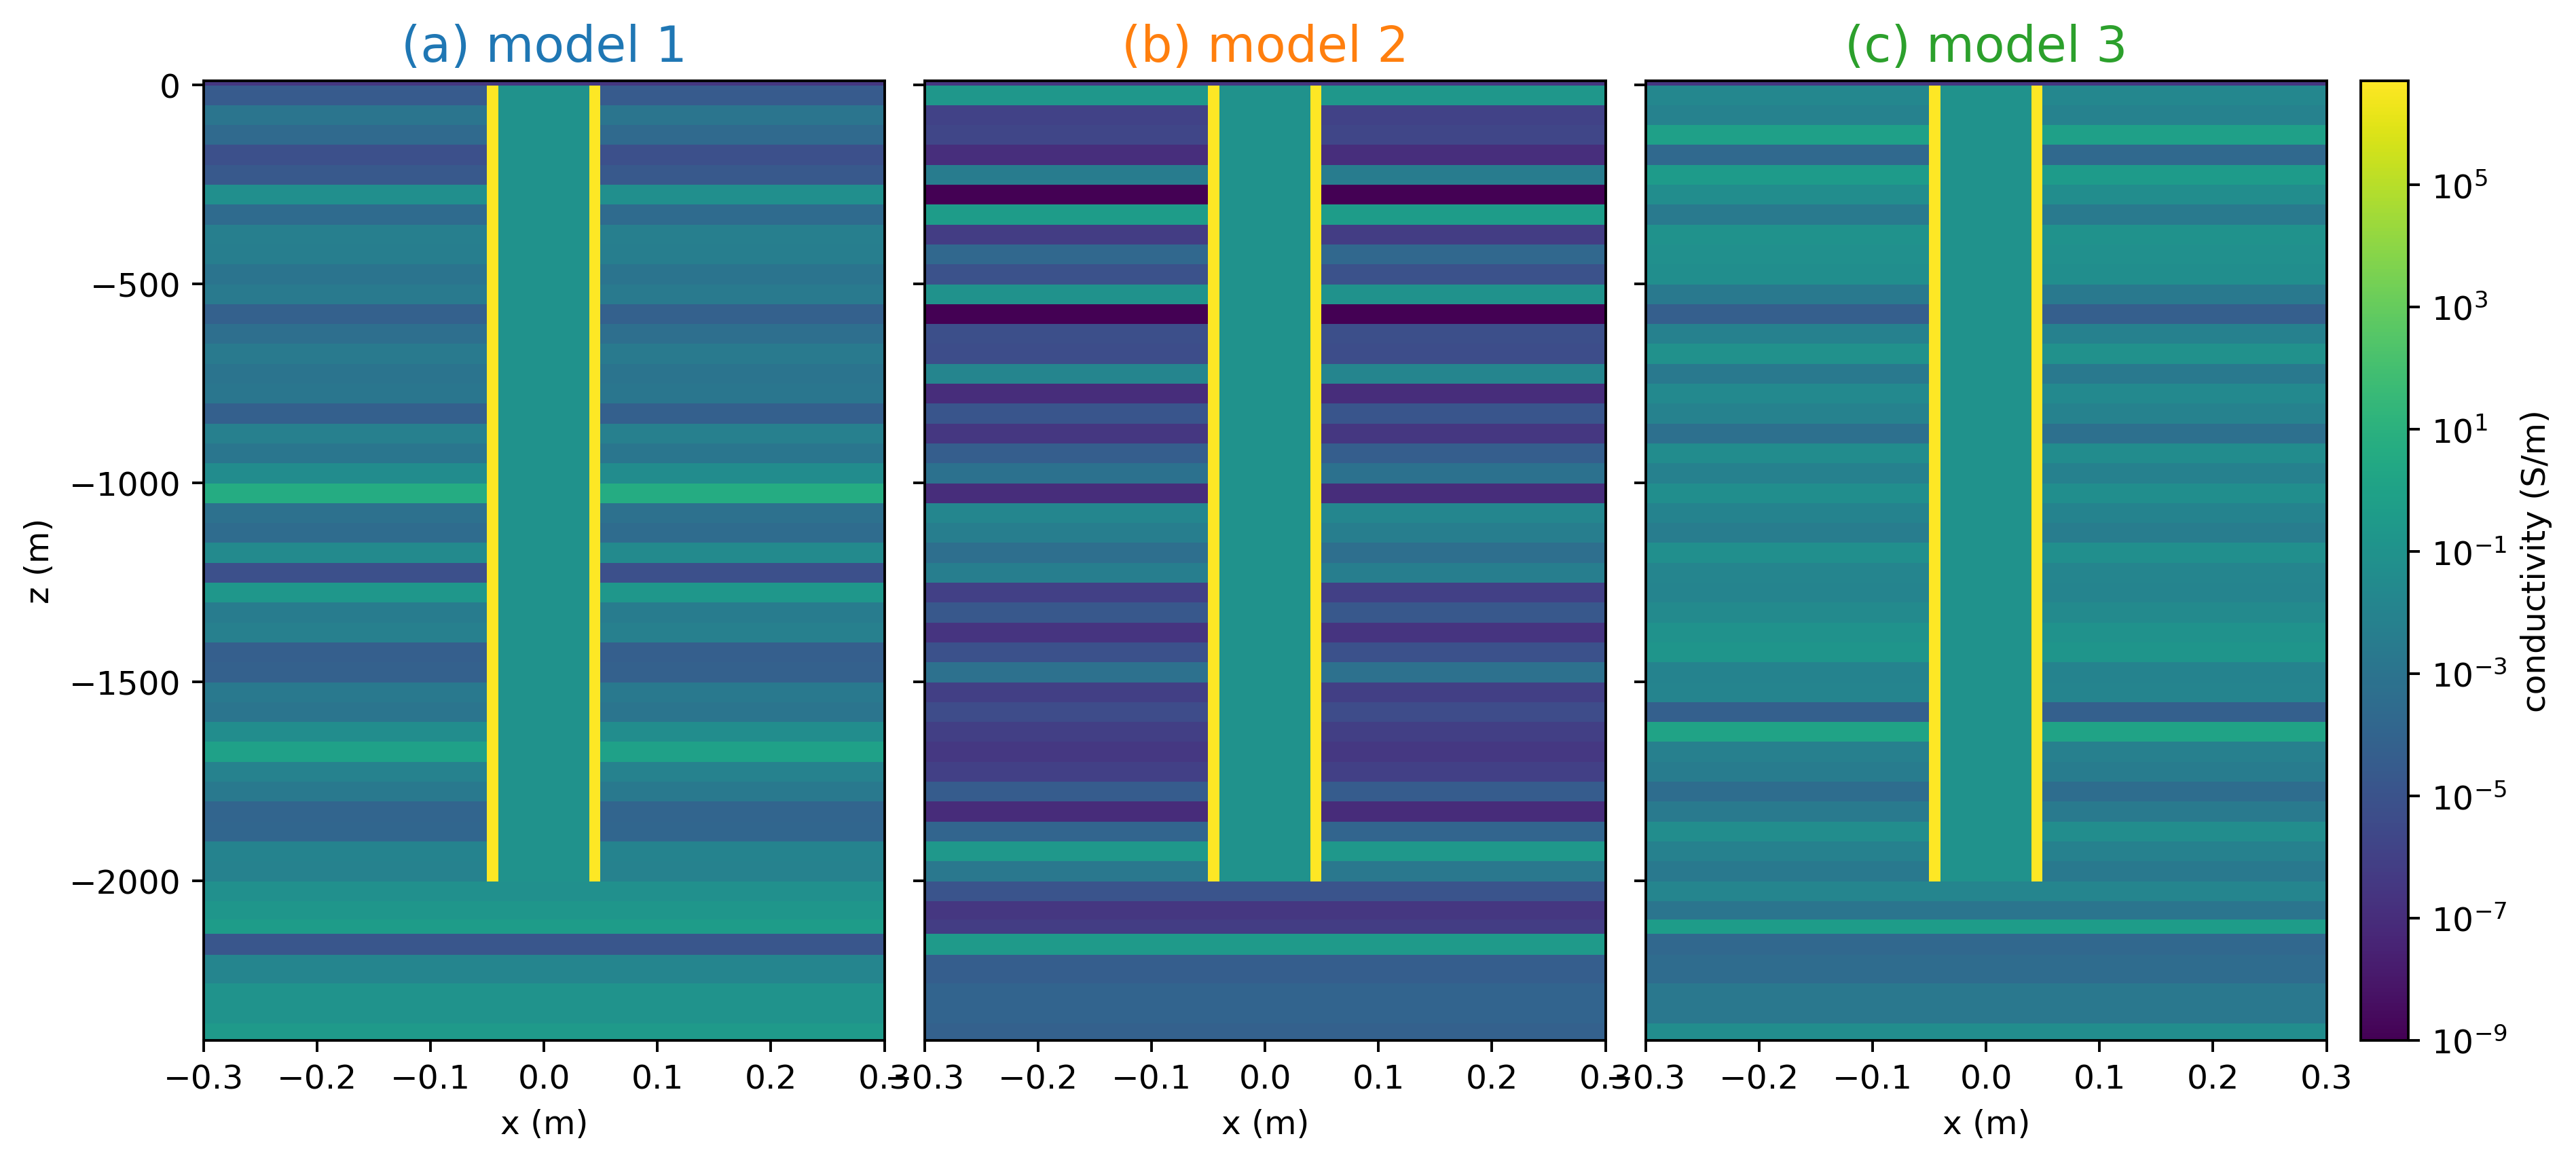
\includegraphics[width=\textwidth]{figures/random_layers.png}
    \end{center}
\caption{
    Three realizations of a 2 km long casing in a layered background, where the conductivity of the
    layers is assigned randomly. Each layer is 50 m thick, and the mean conductivity of the background
    is 0.1 S/m. The color of the title corresponds to the plots of the currents and charges in Figure
    \ref{fig:approximating_wells_currents_charges_random}
}
\label{fig:random_layers}
\end{figure}
